\documentclass{standalone}

\usepackage[latin1]{inputenc}
\usepackage{amsmath}
\usepackage{amssymb}
\usepackage{amsthm}

\usepackage{tikz}
\usetikzlibrary{shapes,arrows,shapes.geometric,calc,patterns}

%% generates a tightly fitting border around the work
%\usepackage[active,tightpage]{preview}
%\PreviewEnvironment{tikzpicture}
%\setlength\PreviewBorder{0.5mm}
%%\renewcommand\PreviewBbAdjust{-\PreviewBorder 1mm -1.15mm -0.85mm}

\usepackage{color}

%\pagestyle{empty}

\begin{document}

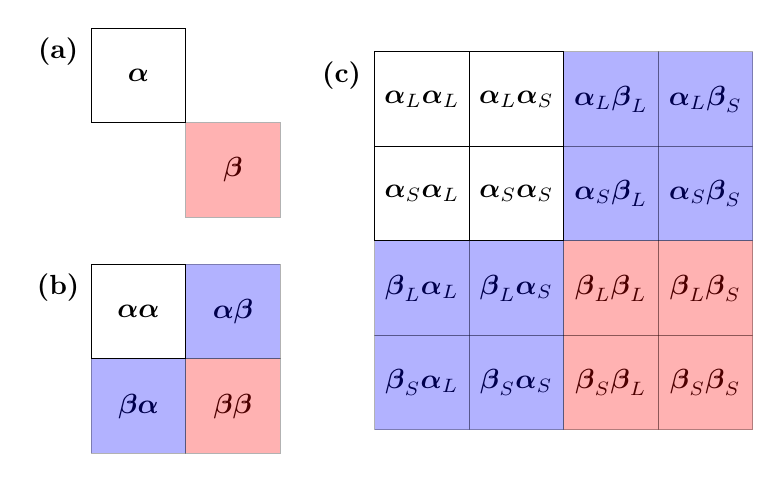
\begin{tikzpicture}[scale=0.6, auto]
  % one-component
  \draw (-0.7,12) node{\textbf{(a)}};
  % alpha
  \draw (1,11.5) node{$\boldsymbol{\alpha}$};
  \draw (0,10.5) rectangle ++(2,2);
  % beta
  \draw (3,9.5) node{$\boldsymbol{\beta}$};
  \draw[fill=red,opacity=0.3] (2,8.5) rectangle ++(2,2);
  % two-component
  \draw (-0.7,7) node{\textbf{(b)}};
  % alpha-alpha
  \draw (1,6.5) node{$\boldsymbol{\alpha\alpha}$};
  \draw (0,5.5) rectangle ++(2,2);
  % alpha-beta
  \draw (3,6.5) node{$\boldsymbol{\alpha\beta}$};
  \draw[fill=blue,opacity=0.3] (2,5.5) rectangle ++(2,2);
  % beta-alpha
  \draw (1,4.5) node{$\boldsymbol{\beta\alpha}$};
  \draw[fill=blue,opacity=0.3] (0,3.5) rectangle ++(2,2);
  % beta-beta
  \draw (3,4.5) node{$\boldsymbol{\beta\beta}$};
  \draw[fill=red,opacity=0.3] (2,3.5) rectangle ++(2,2);
  % four-component
  \draw (5.3,11.5) node{\textbf{(c)}};
  % alpha-alpha
  \draw (7,11) node{$\boldsymbol{\alpha}_{L}\boldsymbol{\alpha}_{L}$};
  \draw (6,10) rectangle ++(2,2);
  \draw (9,11) node{$\boldsymbol{\alpha}_{L}\boldsymbol{\alpha}_{S}$};
  \draw (8,10) rectangle ++(2,2);
  \draw (7,9) node{$\boldsymbol{\alpha}_{S}\boldsymbol{\alpha}_{L}$};
  \draw (6,8) rectangle ++(2,2);
  \draw (9,9) node{$\boldsymbol{\alpha}_{S}\boldsymbol{\alpha}_{S}$};
  \draw (8,8) rectangle ++(2,2);
  % alpha-beta
  \draw (11,11) node{$\boldsymbol{\alpha}_{L}\boldsymbol{\beta}_{L}$};
  \draw[fill=blue,opacity=0.3] (10,10) rectangle ++(2,2);
  \draw (13,11) node{$\boldsymbol{\alpha}_{L}\boldsymbol{\beta}_{S}$};
  \draw[fill=blue,opacity=0.3] (12,10) rectangle ++(2,2);
  \draw (11,9) node{$\boldsymbol{\alpha}_{S}\boldsymbol{\beta}_{L}$};
  \draw[fill=blue,opacity=0.3] (10,8) rectangle ++(2,2);
  \draw (13,9) node{$\boldsymbol{\alpha}_{S}\boldsymbol{\beta}_{S}$};
  \draw[fill=blue,opacity=0.3] (12,8) rectangle ++(2,2);
  % beta-alpha
  \draw (7,7) node{$\boldsymbol{\beta}_{L}\boldsymbol{\alpha}_{L}$};
  \draw[fill=blue,opacity=0.3] (6,6) rectangle ++(2,2);
  \draw (9,7) node{$\boldsymbol{\beta}_{L}\boldsymbol{\alpha}_{S}$};
  \draw[fill=blue,opacity=0.3] (8,6) rectangle ++(2,2);
  \draw (7,5) node{$\boldsymbol{\beta}_{S}\boldsymbol{\alpha}_{L}$};
  \draw[fill=blue,opacity=0.3] (6,4) rectangle ++(2,2);
  \draw (9,5) node{$\boldsymbol{\beta}_{S}\boldsymbol{\alpha}_{S}$};
  \draw[fill=blue,opacity=0.3] (8,4) rectangle ++(2,2);
  % beta-beta
  \draw (11,7) node{$\boldsymbol{\beta}_{L}\boldsymbol{\beta}_{L}$};
  \draw[fill=red,opacity=0.3] (10,6) rectangle ++(2,2);
  \draw (13,7) node{$\boldsymbol{\beta}_{L}\boldsymbol{\beta}_{S}$};
  \draw[fill=red,opacity=0.3] (12,6) rectangle ++(2,2);
  \draw (11,5) node{$\boldsymbol{\beta}_{S}\boldsymbol{\beta}_{L}$};
  \draw[fill=red,opacity=0.3] (10,4) rectangle ++(2,2);
  \draw (13,5) node{$\boldsymbol{\beta}_{S}\boldsymbol{\beta}_{S}$};
  \draw[fill=red,opacity=0.3] (12,4) rectangle ++(2,2);
\end{tikzpicture}

\end{document}
